\documentclass[11pt]{article}

% ---------------------------------------------------------------- packages
\usepackage[letterpaper,margin=1in]{geometry}
\usepackage[T1]{fontenc}
\usepackage{newtxtext}
\usepackage{newtxmath}
\usepackage[protrusion=true,expansion=true]{microtype}
\usepackage{amsmath}
\usepackage{bm}
\usepackage{graphicx}
\usepackage{booktabs}
\usepackage{array}
\usepackage{tabularx}
\usepackage{multirow}
\usepackage{xcolor}
\usepackage{tikz}
\usetikzlibrary{arrows.meta,positioning,calc,fit,backgrounds}
\usepackage[round,authoryear]{natbib}
\usepackage{algorithm}
\usepackage{algpseudocode}
\usepackage[font=small,labelfont=bf,skip=6pt]{caption}
\usepackage{enumitem}
\usepackage{placeins}
\usepackage{float}

% Palette shared with the figures (paper/make_figures.py)
\definecolor{cpblue}{HTML}{2A78D6}
\definecolor{cporange}{HTML}{EB6834}
\definecolor{cpaqua}{HTML}{1BAF7A}
\definecolor{cpink}{HTML}{0B0B0B}
\definecolor{cpinktwo}{HTML}{52514E}
\definecolor{cpmuted}{HTML}{898781}
\definecolor{cpgrid}{HTML}{E1E0D9}
\definecolor{cpaxis}{HTML}{C3C2B7}

\usepackage[colorlinks=true,linkcolor=cpblue!75!black,citecolor=cpblue!75!black,urlcolor=cpblue!75!black]{hyperref}
\usepackage[capitalise,noabbrev]{cleveref}

\setlist{itemsep=2pt,topsep=4pt,parsep=0pt}
\setlength{\parskip}{0pt}

% ---------------------------------------------------------------- notation
\newcommand{\cs}{\textsc{cspredict}}
\newcommand{\model}[1]{\textsc{#1}}
\newcommand{\ci}[2]{{\scriptsize(#1--#2)}}
\newcommand{\pd}[2]{{\scriptsize(#1,\,#2)}}
\newcommand{\norm}{\operatorname{norm}}
\newcommand{\logit}{\operatorname{logit}}
\newcommand{\LL}{\mathrm{LL}}
\newcommand{\1}{\mathbb{1}}

\title{\textbf{Where Are They Now?}\\[4pt]
\Large Calibrated Tracking of Unseen Opponents in \emph{Counter-Strike~2}\\ from Team-Level Information}
\author{Akash Khanikor\\[2pt]
\normalsize Washington University in St.\ Louis\\
\normalsize\texttt{khanikor@wustl.edu}}
\date{September 2026}

\begin{document}
\maketitle

\begin{abstract}
\noindent In tactical shooters such as \emph{Counter-Strike~2} (CS2), most of a round is played against opponents who cannot be seen. We study the problem of estimating, at every moment of a recorded match, a probability distribution over the location of each opponent who has dropped off a team's radar, using only information that team possessed at the time. We present \cs, a factored Bayes filter over a navigation grid learned from player positions (1{,}999 cells grouped into the map's 23 named callouts). Its components are learned from 82 recorded matches on the map \emph{de\_mirage}: a logistic spotting model, fitted on about 27 million observer--enemy pairs, that turns ``a teammate looked here and saw nobody'' into evidence; a particle filter whose particles replay recorded trajectories from similar situations, blended with a grid Markov model and a population prior; learned molotov-avoidance profiles; a coordination correction based on about 134{,}000 recorded snapshots of whole teams; and a post-hoc calibration that depends on how long ago the opponent was last seen. On 16 held-out professional matches (102{,}486 evaluation moments), \cs{} names the correct callout 48.2\% of the time (72.9\% within its top three), against 42.2\% for the common ``they are where I last saw them'' heuristic and 21.3\% for a time-conditioned population prior. Its callout log-loss is 1.663~nats, against 7.196 and 2.607, and its stated probabilities are well calibrated (expected calibration error 0.0010). Ablations attribute most of the gain to replayed trajectories and to negative information, while several intuitive features, such as the weapon an opponent was last seen holding, give no measurable improvement.

\medskip
\noindent\textbf{Keywords:} Bayesian filtering, particle filters, partial observability, negative information, calibration, proper scoring rules, esports analytics.
\end{abstract}

% ================================================================
\section{Introduction}
\label{sec:intro}

\emph{Counter-Strike~2} (CS2) is a five-versus-five tactical shooter. Each player sees only what lies in their own line of sight, plus a shared minimap, the \emph{radar}, that marks any enemy a teammate currently sees. Most of a round is therefore played against opponents whose positions are unknown. Strong players and coaches reason about those positions constantly (``they were last seen on A ramp eight seconds ago, nobody has come through Palace, so they are probably still near the site''), and much of post-match review consists of reconstructing and critiquing exactly this reasoning.

This paper asks whether that reasoning can be made quantitative. Given only what one team knew at a moment of a recorded match, we estimate, for each opponent who has dropped off the radar, a probability distribution over where that opponent is now (\cref{fig:review}). The distributions are meant for demo review. A coach can scrub through a round and see which areas were plausibly occupied, how the uncertainty grew as the team lost track of an opponent, and whether a player's decisions were consistent with the information available at the time.

\begin{figure}[t]
  \centering
  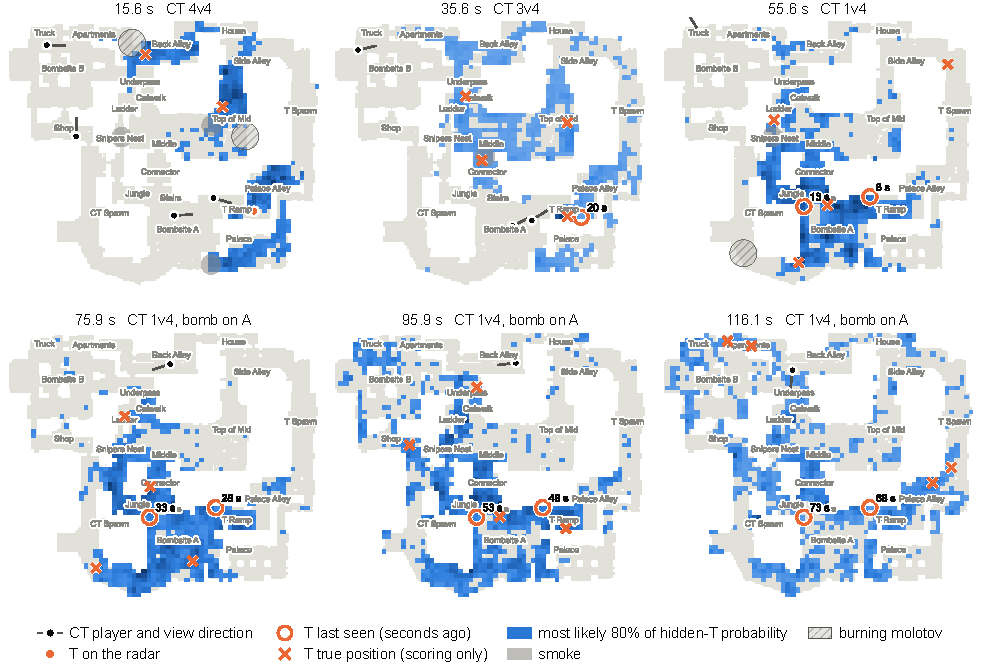
\includegraphics[width=\linewidth]{figures/review.pdf}
  \caption{Six moments of a held-out professional round (EAC vs.\ lilmix, round 9) from the Counter-Terrorist (CT) side, which ends in a 1-versus-4 with the bomb planted on A. Blue cells hold the most likely 80\% of the probability for the hidden Terrorists (Ts), with darker cells more likely. Rings mark where each T was last seen and how long ago. The orange crosses show where the Ts really were; they are drawn for review only and are never seen by the model. Grey discs are smokes and hatched discs burning molotovs.}
  \label{fig:review}
\end{figure}

Four features make the problem harder than it first appears.
\begin{enumerate}[label=(\roman*)]
  \item \textbf{Multimodal uncertainty.} Maps are networks of corridors, so an opponent who may have gone either way is in one corridor or the other, not in the wall between them. A single Gaussian estimate, as in the Kalman filter, describes this poorly.
  \item \textbf{Negative information.} Most of the evidence is the \emph{absence} of a sighting. A teammate who looks down a corridor and sees nobody makes that corridor unlikely, but how unlikely depends on sight lines, distance, the teammate's view direction, smokes and flashes.
  \item \textbf{Situation-dependent behaviour.} How far an opponent travels depends on how long ago they were seen, whether the bomb is planted, the team's economy and the phase of the round.
  \item \textbf{Coordination.} The five opponents act as a team. Tracking each one independently ignores that teams stack a bombsite, send a lurker, or hold a fixed set-up.
\end{enumerate}
In addition, the output must be \emph{calibrated} (when it says 70\%, the opponent should be there about 70\% of the time), and the evaluation must use scores that reward honest probabilities rather than confident guesses.

Our system, \cs, addresses these points with a factored Bayes filter: one belief per opponent over a grid of about two thousand cells, updated every 0.25\,s. Every component is learned from recorded matches. The map's geometry, which we could not obtain, is learned from where players stand. Sight lines and a spotting model are learned from the game's own record of who saw whom. The motion model replays real recorded trajectories from similar situations. A final correction accounts for team coordination and calibrates the output. The closest prior work, by \citet{hladky2008evaluation}, tracked opponents in \emph{Counter-Strike: Source} with 190 LAN games on one map. We revisit the problem with modern professional data, full probability distributions and proper scoring rules.

\paragraph{Contributions.}
\begin{itemize}
  \item A formulation of opponent tracking from team-level information in CS2, with an information state restricted to what the team could know, and an evaluation protocol based on proper scoring rules, round-level bootstrap intervals and paired comparisons (\cref{sec:problem,sec:setup}).
  \item A complete filter learned from demo files alone. It needs no map geometry and combines a logistic spotting model for negative information with a trajectory-library particle filter conditioned on the time since the last sighting (\cref{sec:method}).
  \item A coordination correction that sums over every pairing between tracked opponents and recorded team snapshots, and a calibration that depends on the forecast horizon. We show why the former must wait for first contact and why the latter must depend on the horizon (\cref{sec:team,sec:calibration,sec:discussion}).
  \item An empirical study on 16 held-out professional matches, with ablations of every component, features that did \emph{not} help, and a comparison with a general-purpose model queried through text descriptions (\cref{sec:results}).
\end{itemize}

The intended use is post-match analysis. Used live during a match, a tool like this would give players information they are not entitled to, which competitive platforms forbid (\cref{sec:limitations}).

% ================================================================
\section{Background and Related Work}
\label{sec:background}

\subsection{Bayesian filtering}
A \emph{Bayes filter} tracks a hidden state $x_t$, here an opponent's position, from a sequence of observations $z_{1:t}$ \citep{thrun2005probabilistic}. It maintains a \emph{belief} $b_t(x) = P(x_t = x \mid z_{1:t})$ and alternates two steps:
\begin{align}
  \text{predict:}\quad & \bar b_t(x) = \sum_{x'} P(x_t = x \mid x_{t-1} = x')\, b_{t-1}(x'), \label{eq:predict}\\
  \text{update:}\quad & b_t(x) = \frac{P(z_t \mid x_t = x)\, \bar b_t(x)}{\sum_{x''} P(z_t \mid x_t = x'')\, \bar b_t(x'')}. \label{eq:update}
\end{align}
The prediction spreads the belief according to a \emph{motion model}; the update is Bayes' rule with an \emph{observation model} $P(z_t \mid x_t)$. When the dynamics are linear and all noise is Gaussian, the belief stays Gaussian and the filter reduces to the Kalman filter \citep{kalman1960new}. For multimodal beliefs one either discretizes the state (a \emph{grid} or histogram filter) or represents the belief by weighted samples (a \emph{particle filter}; \citealp{gordon1993novel,kitagawa1996monte,doucet2001sequential}). Particle filters periodically \emph{resample}, duplicating heavy particles and dropping light ones, when the effective sample size $1/\sum_m w_m^2$ of the normalized weights falls too low \citep{kong1994sequential}.

Updating on the \emph{failure} to detect a target, known as negative information, is classical in search theory \citep{stone1975theory}. If a sensor would detect a target at $x$ with probability $\pi(x)$ and reports nothing, the likelihood of that report is $1 - \pi(x)$, which removes probability from well-covered places. \Cref{fig:concept} illustrates one predict--update cycle of this kind.

\begin{figure}[t]
\centering
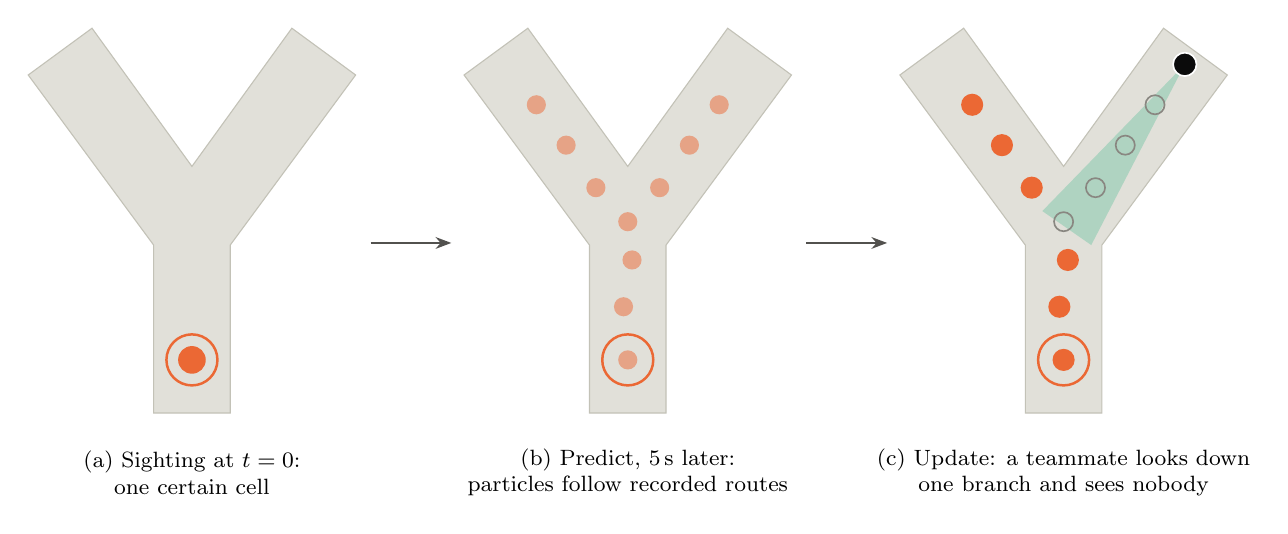
\begin{tikzpicture}[x=0.27mm, y=-0.27mm, font=\footnotesize]
  \foreach \dx in {0,205,410} {
    \begin{scope}[shift={(\dx,0)}]
      \filldraw[fill=cpgrid, draw=cpaxis, line width=0.4pt] (72,190) -- (72,111) -- (13,31) -- (43,9) -- (90,74) -- (137,9) -- (167,31) -- (108,111) -- (108,190) -- cycle;
      \draw[cporange, line width=0.9pt] (90,165) circle (12);
    \end{scope}
  }
  % (a) the sighting
  \fill[cporange] (90,165) circle (6.5);
  % (b) predicted particles
  \begin{scope}[shift={(205,0)}]
    \foreach \x/\y in {90/165, 88/140, 92/118, 90/100, 75/84, 61/64, 47/45, 105/84, 119/64, 133/45}
      \fill[cporange, opacity=0.5] (\x,\y) circle (4.5);
  \end{scope}
  % (c) after the teammate's null observation
  \begin{scope}[shift={(410,0)}]
    \fill[cpaqua, opacity=0.25] (147,26) -- (80,95) -- (103,111) -- cycle;
    \foreach \x/\y in {90/100, 105/84, 119/64, 133/45}
      \draw[cpmuted, line width=0.6pt] (\x,\y) circle (4.5);
    \foreach \x/\y in {90/165, 88/140, 92/118, 75/84, 61/64, 47/45}
      \fill[cporange] (\x,\y) circle (5.2);
    \filldraw[fill=cpink, draw=white, line width=0.6pt] (147,26) circle (5.5);
  \end{scope}
  \draw[-{Stealth[length=2mm]}, cpinktwo, line width=0.6pt] (174,110) -- (212,110);
  \draw[-{Stealth[length=2mm]}, cpinktwo, line width=0.6pt] (379,110) -- (417,110);
  \node[align=center] at (90,218) {(a) Sighting at $t = 0$:\\ one certain cell};
  \node[align=center] at (295,218) {(b) Predict, 5\,s later:\\ particles follow recorded routes};
  \node[align=center] at (500,218) {(c) Update: a teammate looks down\\ one branch and sees nobody};
\end{tikzpicture}
\caption{One predict--update cycle, schematically. An enemy is seen at the foot of a forked corridor (orange ring). As time passes, the belief (orange dots, each a particle carrying probability) spreads along the routes players really take. A teammate (black dot) then looks down the right branch (green wedge) and reports nothing. The particles in view lose their weight (grey circles), and after renormalization the remaining probability, in the left branch and the corridor, grows.}
\label{fig:concept}
\end{figure}

Our particle motion model follows \emph{analog forecasting} \citep{lorenz1969atmospheric}. Instead of a parametric motion model, each particle follows a recorded trajectory that passed through a situation similar to the current one. This is a kernel-weighted nearest-neighbour method \citep{cover1967nearest} applied to whole futures rather than to single labels.

\subsection{Opponent modelling in games}
The problem of locating hidden opponents appears across game genres. \citet{isla2006probabilistic} describes \emph{occupancy maps}: a probability grid that diffuses over a level and is erased wherever the agent can see, which is our \model{Diffuse} baseline. \citet{bererton2004state} proposed particle filters for game AI, and \citet{weber2011particle} learned particle models from expert \emph{StarCraft} replays. \citet{synnaeve2018forward} and \citet{jeong2020defoggan} predict hidden \emph{StarCraft} units with neural encoder--decoders and generative adversarial networks. \citet{tastan2012learning} combined learned motion models with particle filters to intercept opponents in \emph{Unreal Tournament}. OpenAI Five handled fog of war in \emph{Dota~2} partly by reusing the last observation of unseen heroes \citep{berner2019dota}, which is our \model{LastSeen} baseline. See \citet{yannakakis2018artificial} for a broader survey.

For Counter-Strike specifically, \citet{hladky2008evaluation} and \citet{hladky2009predicting} built per-opponent hidden semi-Markov models and particle filters for \emph{Counter-Strike: Source}. Their observation model used negative information from the friendly team's field of view. Trained on 140 LAN games on one map and evaluated on 50, their models matched or exceeded human experts at predicting where Terrorists were. They produced point predictions evaluated by path distance, modelled opponents independently, and did not condition on game state such as economy. Recent work on CS2 approaches the question from other angles. X-Ego \citep{wang2025xego} predicts which callouts contain opponents from first-person video with the minimap masked out; we use its recordings as a second data source. MLMove \citep{durst2024learning} learns professional movement for bots from observations of all ten players, and \citet{xenopoulos2020valuing} and the ESTA dataset \citep{xenopoulos2022esta} support win-probability and player-valuation models. None of these produces a calibrated belief over hidden opponents from team-level information.

\subsection{Evaluating probabilistic forecasts}
A scoring rule is \emph{proper} if a forecaster minimizes its expected score by reporting their true beliefs \citep{gneiting2007strictly}. The logarithmic score \citep{good1952rational} and the Brier score \citep{brier1950verification} are proper. Rules such as ``probability within 300 units of the truth'' are not, and they reward over-confident point guesses (\cref{app:improper}). A forecaster is \emph{calibrated} if events it assigns probability $p$ happen with frequency $p$ \citep{degroot1983comparison}. Calibration is usually checked with reliability diagrams and summarized by the expected calibration error \citep{naeini2015obtaining}, and it can be repaired after the fact by monotone maps such as Platt scaling \citep{platt2000probabilities} or temperature scaling \citep{guo2017calibration}. For uncertainty intervals we use the bootstrap \citep{efron1979bootstrap,efron1993introduction}, resampling whole rounds as clusters because moments within a round are strongly dependent \citep{field2007bootstrapping}.

% ================================================================
\section{Problem Formulation}
\label{sec:problem}

\paragraph{Map and time.} We discretize the walkable area of the map into cells $i \in \mathcal{V} = \{1, \dots, N\}$ with $N = 1{,}999$ (\cref{sec:grid}). A labelling $c: \mathcal{V} \to \mathcal{C}$ assigns every cell to one of $|\mathcal{C}| = 23$ \emph{callouts}, the named regions players use to communicate (\emph{Jungle}, \emph{Palace}, \emph{Bombsite~A}, \dots). Time advances in steps of $\Delta = 0.25$\,s from the end of the round's freeze time. Positions are in game units; for scale, a standing player is 72~units tall and 32~wide, and running speeds are roughly 200--250~units/s.

\paragraph{Information state.} Fix a round and a \emph{friendly} side; the other side's players are the \emph{enemies} $e \in \mathcal{E}$, $|\mathcal{E}| \le 5$. At step $t$ the friendly team's information $\mathcal{I}_t$ consists of:
\begin{itemize}
  \item the position, yaw and pitch of every friendly player, and whether they are alive or blinded by a flashbang;
  \item for every enemy, whether it is on the radar and, if so, its cell $y^e_t \in \mathcal{V}$ (otherwise $y^e_t = \varnothing$) and the weapon in its hands;
  \item active smokes and burning molotovs or incendiaries;
  \item the kill feed (who killed whom and with which weapon, whether through a wall or smoke) and where friendly victims died;
  \item which enemies are alive and which rounds each team has won (the scoreboard), the round clock, and the bomb phase $\phi_t \in \{0, 1, 2\}$ (not planted, planted on A, planted on B).
\end{itemize}
The demo file also records every enemy's true position $x^e_t$. These positions are withheld from the model and used only for scoring.

\paragraph{Task.} For each alive enemy not on the radar, compute
\begin{equation}
  b^e_t(i) = P\big(x^e_t = i \mid \mathcal{I}_{1:t}\big), \qquad q^e_t(k) = \sum_{i:\, c(i) = k} b^e_t(i),
\end{equation}
the cell belief and the implied \emph{callout belief}. We denote by $\tau^e_t$ the seconds since enemy $e$ was last on the radar ($\tau = \infty$ if never this round). Our evaluation targets the mid- and late-round case, meaning moments when an enemy is off the radar \emph{but was seen earlier in the round}. Before first contact the best available answer is essentially ``where that side usually goes,'' which a population prior already provides; those moments are reported separately.

\paragraph{Assumptions.} We assume, as the game's interface makes largely true, that the team can tell which enemy it is seeing on the radar, and that burning molotovs are known to both teams: the thrower saw where it landed, and the flames are visible and audible. The opponents' economy class (eco, force buy or full buy) shapes how they play, but their money and equipment values are hidden. The model therefore estimates the class from the round history and the guns the team has seen, on the radar or in the kill feed (\cref{sec:infostate}). The estimate names the right class for 77\% of validation rounds when freeze time ends, and at 92\% of the validation moments we evaluate, by when guns have been seen. Earlier versions of the model took the class from the actual equipment values. Doing so instead changes callout log-loss by $+0.001$ ($-0.007$ to $+0.008$) on validation, averaged over two random seeds of the particle filter, and by $+0.002$ ($-0.004$ to $+0.008$) on test; top-1 accuracy changes by $0.000$ ($-0.002$ to $+0.002$) and $-0.001$ ($-0.004$ to $+0.001$). Rerunning the particle filter with another random seed moves both metrics as much. We do not use sound (footsteps, gunfire), by design; \cref{sec:limitations} discusses this choice.

% ================================================================
\section{Data}
\label{sec:data}

We use two sources of recorded CS2 matches on the map \emph{de\_mirage} (\cref{tab:data}). \textbf{HLTV (professional):} 71 maps, one from each of 71 series, downloaded manually from HLTV.org \citep{hltv} in September 2026. The events include CCT, ESEA, ESL Challenger League, iBuyPower Masters and Stake Pulse, so most teams are tier two or three, with some tier one. \textbf{FACEIT (development):} the 46 Mirage matches of the X-Ego-CS dataset \citep{wang2025xego}, played between players ranked in the top 100 on the FACEIT platform, with the dataset's own train/validation/test split. The FACEIT matches were recorded on an earlier game patch (14094 against 14181--14185), but the Mirage layout is unchanged: 99.9\% of professional positions fall on cells already mapped from the FACEIT data.

Demos record the game state at 64 ticks per second. We parse them with demoparser2 and awpy \citep{demoparser,awpy}, keep every eighth tick (8\,Hz), and run the filter every 16 ticks (0.25\,s). For each player we keep position, view angles, alive status, equipment value, the active weapon, the game's place name for the current position, and the game's own radar state: a per-player \emph{spotted} flag and a \emph{spotted-by} list of the opponents who currently see that player. Events include kills (with wallbang and through-smoke flags), bomb plants, smokes, infernos and flashbangs.

Four data problems had to be solved along the way, and each is documented because it changed results. (1)~awpy's download server for map geometry, navigation meshes and collision triangles returned errors, so the geometry had to be learned from player positions (\cref{sec:grid}). (2)~Without that geometry, awpy labels every bomb plant as bombsite~B; we relabel each plant with the nearer bombsite, whose centre is the mean position of players standing where the game's place name is Bombsite~A or Bombsite~B. (3)~A parsing bug cut 15\% of smokes 4\,s short. (4)~55 of the 71 HLTV demos contain no \texttt{player\_blind} events, so flashed players looked able to spot. We reconstruct flashes from each player's networked flash duration, which jumps to exactly the event's blind duration on the tick of the flash; on demos that contain both, the reconstruction reproduces every event that names a player.

Splits are made by whole maps, so no round of a test map is ever seen in training. HLTV maps are assigned 70/10/20\% to training, validation and test by a stable hash of the demo identifier, which gives 47/8/16 maps. Models are trained on the 82 pooled training maps (47~HLTV and 35~FACEIT), all settings are chosen on validation maps, and the 16 HLTV test maps are used only to report results.

\begin{table}[t]
\centering
\caption{Data. Each map is one game of a series; the two teams swap sides at half time, and a match on Mirage is up to 24 rounds plus overtime. Evaluation moments are (step, hidden enemy) pairs with the enemy seen earlier in the round, pooled over both teams' viewpoints.}
\label{tab:data}
\small
\begin{tabular}{@{}lcc@{}}
\toprule
 & HLTV (professional) & FACEIT (X-Ego-CS) \\
\midrule
Maps: train / validation / test & 47 / 8 / 16 \;(71) & 35 / 5 / 6 \;(46) \\
Rounds: train / validation / test & 1{,}030 / 171 / 329 \;(1{,}530) & 793 / 107 / 132 \;(1{,}032) \\
Players & tier-2/3 professionals, some tier 1 & top-100 FACEIT players \\
Game patch & 14181--14185 & 14094 \\
Split & stable hash of the demo id & provided with the dataset \\
Evaluation moments & 63{,}906 (validation), 102{,}486 (test) & 48{,}876 (test) \\
\bottomrule
\end{tabular}
\end{table}

% ================================================================
\section{Method}
\label{sec:method}

\Cref{fig:pipeline} gives an overview. Offline, we fit a navigation grid, a spotting model, two motion models, molotov profiles, a library of team snapshots and an economy estimate on the training maps, and a calibration map on the validation maps. Online, the filter reconstructs what the team knew and runs a predict--update step for every hidden enemy every 0.25\,s, followed by output-only corrections. \Cref{alg:step} summarizes one step, and \cref{app:hyper} lists every constant.

\begin{figure}[t]
\centering
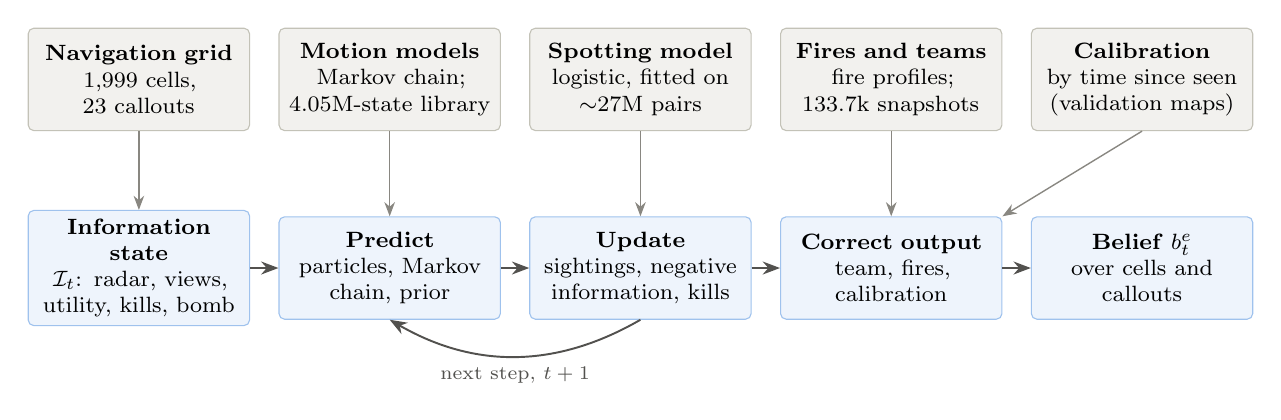
\begin{tikzpicture}[
  font=\footnotesize,
  box/.style={draw=cpaxis, rounded corners=2pt, align=center, minimum height=1.3cm, text width=2.6cm, inner sep=3pt},
  off/.style={box, fill=cpgrid!45},
  on/.style={box, fill=cpblue!8, draw=cpblue!45},
  flow/.style={-{Stealth[length=2.2mm]}, line width=0.7pt, cpinktwo},
  feed/.style={-{Stealth[length=1.8mm]}, line width=0.5pt, cpmuted},
  node distance=0.36cm]
  \node[off] (grid) {\textbf{Navigation grid}\\ 1{,}999 cells,\\ 23 callouts};
  \node[off, right=of grid] (motion) {\textbf{Motion models}\\ Markov chain;\\ 4.05M-state library};
  \node[off, right=of motion] (spot) {\textbf{Spotting model}\\ logistic, fitted on\\ $\sim$27M pairs};
  \node[off, right=of spot] (aux) {\textbf{Fires and teams}\\ fire profiles;\\ 133.7k snapshots};
  \node[off, right=of aux] (cal) {\textbf{Calibration}\\ by time since seen\\ (validation maps)};
  \node[on, below=1.0cm of grid] (info) {\textbf{Information state}\\ $\mathcal{I}_t$: radar, views,\\ utility, kills, bomb};
  \node[on, right=of info] (pred) {\textbf{Predict}\\ particles, Markov\\ chain, prior};
  \node[on, right=of pred] (upd) {\textbf{Update}\\ sightings, negative\\ information, kills};
  \node[on, right=of upd] (post) {\textbf{Correct output}\\ team, fires,\\ calibration};
  \node[on, right=of post] (out) {\textbf{Belief} $b^e_t$\\ over cells and\\ callouts};
  \draw[flow] (info) -- (pred);
  \draw[flow] (pred) -- (upd);
  \draw[flow] (upd) -- (post);
  \draw[flow] (post) -- (out);
  \draw[flow] (upd.south) to[out=-150, in=-30] node[below, font=\scriptsize, text=cpinktwo] {next step, $t+1$} (pred.south);
  \draw[feed] (grid) -- (info);
  \draw[feed] (motion) -- (pred);
  \draw[feed] (spot) -- (upd);
  \draw[feed] (aux) -- (post);
  \draw[feed] (cal.south) -- (post.north east);
\end{tikzpicture}
\caption{System overview. Grey boxes are fitted once; blue boxes run at every filter step. Grey arrows show the main fitted component each online stage uses; the fire profiles also reshape the grid chain's predictions. The output corrections reshape only the reported belief and never feed back into the recursion.}
\label{fig:pipeline}
\end{figure}

\subsection{Reconstructing the information state}
\label{sec:infostate}
An enemy is \emph{on the radar} during a step if its spotted flag is set at either of the step's two 8\,Hz samples, and its sighting cell is the most recent one. A friendly player can spot only while alive and not blinded; a flash counts as blinding when it lasts more than 0.3\,s, from the flash until its duration expires. Smokes block sight from 1.0\,s after they burst until 1.5\,s before they expire. We measured both offsets from spotting rates through smokes in the training demos, since a smoke needs time to bloom and thins out before it disappears. Molotovs count as burning from 0.5\,s after they burst, when the flames have spread, until they burn out. A kill by an enemy is attached to the first step at or after it, together with the victim's position and whether it went through a wall or a smoke. A team's economy is summarized by its mean equipment value when freeze time ends: an \emph{eco} below 1{,}500, a \emph{force buy} up to 3{,}800, and a \emph{full buy} above that. Recorded rounds carry this class, but the friendly team cannot see its opponents' equipment, so for the round being tracked the class is estimated from public information (\cref{sec:problem}). The prior is how often each class was bought in the training rounds in the same economic situation, smoothed with 3 rounds at the overall frequencies. The situations are the pistol round, overtime, round~2 by the pistol-round result, round~3 after a loss in round~2 (again by the pistol-round result), any other round after a win, and any other round after a loss by its loss-bonus count (one up per round lost in the half, one down per round won, at most 4). Each enemy seen so far multiplies the prior by the probability, under each class, of the dearest gun that enemy has shown on the radar or in the kill feed (pistol, SMG, rifle or sniper), raised to the power 0.7 because teammates buy together. The economy factors of the matching kernels below ($0.7$ per class of difference) are averaged over this estimated distribution of the opponents' class.

\subsection{A navigation grid learned from player positions}
\label{sec:grid}
Without map geometry, we learn the walkable space from where players have stood (\cref{fig:grid}a). The map is cut into columns of $64 \times 64$ units. Within a column, the recorded heights are split into floors wherever consecutive heights differ by more than 110~units (a jump reaches about 66), and every floor with at least one second of recorded presence becomes a cell. A column can hold several floors, as where Underpass runs beneath Catwalk. Cells are joined by an edge if players were seen moving directly between them at least twice, or if they are horizontal neighbours whose floors differ by at most 48~units. Keeping the largest connected component leaves $N = 1{,}999$ cells and 6{,}780 edges. Each cell takes the most common game place name among the positions recorded in it, which gives the 23 callouts, and a representative standing point (the mean recorded position, moved onto a walked spot). Walking distances between cells are shortest paths on this graph. A finer $16 \times 16$-unit raster records which spots were ever walked on, and at what heights, for the ray casting below.

\begin{figure}[t]
  \centering
  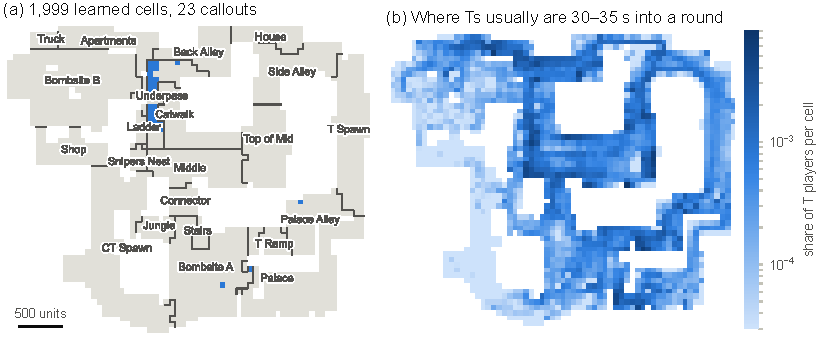
\includegraphics[width=\linewidth]{figures/grid.pdf}
  \caption{(a) The navigation grid learned from player positions. Lines separate callouts (on the lower floor), and blue marks the 27 map columns that hold two floors, mostly Catwalk above Underpass. (b) The population prior used as a baseline and as 10\% of the ensemble: where Terrorists stand 30--35\,s into a round before the bomb is planted, pooled over the training maps (log scale).}
  \label{fig:grid}
\end{figure}

\subsection{Observation model: who would have seen whom}
\label{sec:spot}
The core of the observation model is the probability $\pi_o(i)$ that friendly observer $o$ would have an enemy standing in cell $i$ on the radar. We model it with a logistic regression \citep{hastie2009elements} on binned features:
\begin{equation}
  \logit \pi_o(i) = \alpha_{s(o,i),\, d(o,i)} + \beta_{h(o,i)} + \gamma_{v(o,i)},
  \label{eq:spot}
\end{equation}
where $d$ is one of eight distance bins (edges at 250, 500, 750, 1{,}000, 1{,}500, 2{,}000 and 3{,}000 units), $h$ and $v$ are the horizontal and vertical angles between the observer's view direction and the target's chest (48~units above the floor) in 5-degree bins, and $s$ is a sight-line class from two ray casts, precomputed for every pair of cells, between the eye points (64~units above the floor) of the observer's cell and the target's cell. The \emph{walk} ray cast treats every raster pixel nobody ever stood on as a wall, and also blocks rays that pass below rising terrain or through the slab of an upper floor. It is precise but closes open areas that nobody walks, such as the air above a drop. The \emph{carve} ray cast additionally opens every pixel through which a \emph{real} spotting ray, from an observer's eyes to the spotted enemy's chest, passed at a similar height, since every recorded sighting proves its sight line was clear. Every walk-clear line is also carve-clear, so $s$ takes three values: clear in both, clear only after carving, or blocked.

The coefficients are fitted by maximum likelihood with a small $L_2$ penalty, using L-BFGS \citep{byrd1995limited}, on aggregated counts over about 27 million observer--enemy pairs from the training demos, excluding pairs hidden by a smoke or a flash. The fitted model separates spotted from unspotted pairs with a held-out area under the ROC curve of 0.99: given one pair where spotting happened and one where it did not, it ranks the former higher 99\% of the time \citep{hanley1982meaning}. The additive model cannot know about individual windows or boxes, so it is multiplied by a per-cell-pair correction, an empirical-Bayes ratio of observed to expected sightings shrunk towards 1 with 3~pseudo-counts \citep{efron1975data}. Pairs of cells that never appeared together therefore keep the geometric estimate. Finally, a sight line passing within 130~units of an active smoke is blocked, and $\pi_o(i)$ is capped at 0.9 so that no cell is ever treated as certainly empty.

\Cref{fig:spot} shows the fitted terms. Spotting falls steeply with distance and with the angle off the view direction. The peak within 5 degrees probably reflects, in part, reverse causation: players turn their crosshair towards enemies they have seen.

\begin{figure}[t]
  \centering
  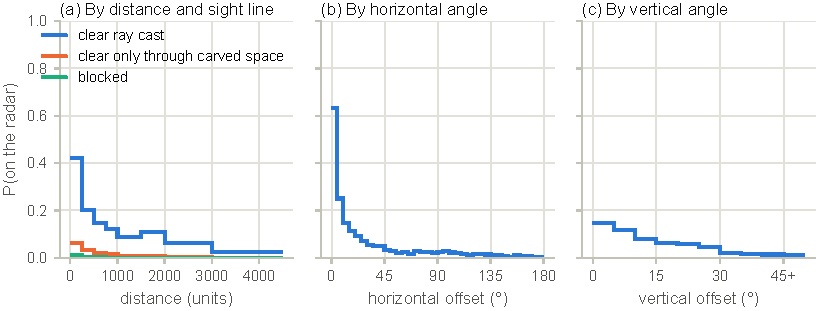
\includegraphics[width=\linewidth]{figures/spot.pdf}
  \caption{The fitted spotting model, as the probability that an enemy standing in a cell is on the radar at a sampled tick, before the per-pair correction. (a) By distance and sight-line class, for a target 10--15$^\circ$ off the view direction horizontally and within 5$^\circ$ vertically. (b) By horizontal offset, for a clear sight line at 500--750 units. (c) By vertical offset, same conditions as (a) at 500--750 units.}
  \label{fig:spot}
\end{figure}

\paragraph{Negative information.} An alive enemy who is not on the radar is evidence against every cell the team could see. Assuming observers detect independently given the enemy's cell,
\begin{equation}
  L_t(i) = P(\text{enemy not on the radar} \mid x_t = i) = \prod_{o \in \mathcal{O}_t} \big(1 - \pi_o(i)\big),
  \label{eq:neg}
\end{equation}
where $\mathcal{O}_t$ is the set of alive, unblinded friendly players. The update of \cref{eq:update} multiplies the belief by $L_t^{\gamma}$; a tempering exponent $\gamma < 1$ would soften the evidence, but $\gamma = 1$ was best on validation.

\paragraph{Kill feed.} When an enemy kills a friendly player, the killer must have had a line of sight to where the victim died. We weight cell $i$ by $K(i) = 0.05 + 0.95\,\tilde\pi(i) / \max_j \tilde\pi(j)$, where $\tilde\pi(i)$ is the spotting probability between the victim's cell and $i$ with the view-angle terms at their best. For wallbangs and kills through smoke only range is used: $K(i) = 1$ within 2{,}000 units and 0.05 beyond. The floor of 0.05 keeps a mistaken likelihood from eliminating the truth.

\subsection{Motion models}
\label{sec:motion}

\paragraph{Grid Markov chain (\model{HMM}).} A first-order Markov chain over cells, one step per 0.25\,s, is estimated by counting recorded transitions $C_{ij}$ between consecutive steps of every alive player. The transition matrix is conditioned on the enemy's side $\varsigma$ (T or CT), the bomb phase $\phi$, and a bin $\tau$ of the time since the player was last on the opponents' radar: 0--2, 2--5, 5--10, 10--20 or more than 20 seconds, or never this round. Players who were just seen tend to hold or fall back, while players unseen for a while rotate along routes. Rare contexts would give noisy estimates, so each level is shrunk towards the one above it:
\begin{equation}
  T^{(\varsigma,\phi)} = \norm\!\big(C^{(\varsigma,\phi)} + 0.5\, S\big), \qquad
  T^{(\varsigma,\phi,\tau)} = \norm\!\big(C^{(\varsigma,\phi,\tau)} + 4\, T^{(\varsigma,\phi)}\big),
  \label{eq:shrink}
\end{equation}
where $\norm$ normalizes rows to sum to one and $S = \norm(I + A)$ spreads pseudo-counts over each cell and its grid neighbours ($A$ is the adjacency matrix). Adding $\lambda$ times a stochastic matrix adds $\lambda$ pseudo-observations to each row, distributed like the parent model. The prediction step is $\bar b_t = b_{t-1} T^{(\varsigma,\phi_t,\tau_t)}$.

\paragraph{Trajectory-library particles (\model{PF}).} A first-order chain forgets a player's heading at every step, so its predictions spread diffusively, while real players run along routes: ten seconds after a sighting they can be 2{,}000 units away. Our second motion model therefore replays real trajectories. The \emph{library} holds every recorded state of every alive player in the training rounds at 0.25\,s spacing, 4{,}054{,}305 states in 18{,}197 trajectories. Each state stores its cell, round time, bomb phase, time since that player was last spotted, team economy, velocity, and a pointer to the next state of the same trajectory. Each enemy is tracked by $M = 512$ particles, each a pointer $\ell_m$ into the library with a weight $w_m$. At every step a particle simply advances to the next state of its recording, $\ell_m \leftarrow \mathrm{next}(\ell_m)$.

When the enemy is sighted in cell $j$, all particles are redrawn from library states of players on the enemy's side in $j$ (widening to up to three rings of neighbouring cells if fewer than 40 states are there). Candidate $\ell$ is drawn with probability proportional to a product of similarity kernels:
\begin{equation}
  \kappa(\ell) = \exp\!\Big(-\frac{(t_\ell - t)^2}{2 \cdot 15^2}\Big) \cdot 0.02^{\1[\phi_\ell \neq \phi_t]} \cdot \exp\!\Big(-\frac{(\ln(1+\tau_\ell) - \ln(1+\tau))^2}{2 \cdot 0.5^2}\Big) \cdot 0.7^{|\mathrm{buy}_\ell - \mathrm{buy}|} \cdot k_v(\ell),
  \label{eq:kernel}
\end{equation}
with round time $t$ in seconds and $\tau$ the time since last seen (the $\tau$ kernel is replaced by 0.05 when exactly one of the two states has never been seen). The heading kernel $k_v$ compares the enemy's velocity $v$ with the candidate's velocity $v_\ell$. It is used only when the enemy was also seen within the previous 0.5\,s, so that $v$ can be measured; otherwise, as on a first sighting, $k_v = 1$. If both move faster than 80~units/s, it is a von Mises kernel $\exp(3(\cos\theta_\ell - 1))$ in the angle between them \citep{mardia2000directional}. It is 0.3 for a stationary candidate when the enemy moves, and $\exp(-|v_\ell|/15)$, with speeds in units per step, when the enemy stands still. On later steps the weights absorb the evidence: $w_m \leftarrow w_m\, L_t(\mathrm{cell}(\ell_m))\, K_t(\mathrm{cell}(\ell_m))$, then renormalize. When the effective sample size $1/\sum_m w_m^2$ falls below $M/3$, the particles are resampled systematically. Duplicated particles are then re-matched to fresh recordings from their current state, so that copies do not share one future. A particle whose recording ends (the player died or the round ended) is re-matched the same way. The belief is the weighted histogram of particle cells, smoothed over two rings of neighbours ($0.4\,\hat b + 0.4\,\hat b P + 0.2\,\hat b P^2$ with $P$ the neighbour-averaging matrix), since 512 particles are a sparse sample of 1{,}999 cells.

The matching kernel deliberately omits some variables. Matching also on the numbers alive on each side, on the same player's own trajectories, or on the weapon last seen was tried and did not help (\cref{sec:negative}).

\paragraph{Baselines.} \model{LastSeen} keeps all probability on the last sighting. \model{Prior} ignores all evidence and uses where that side's players stand, by bomb phase and 5-second bin of round time, in the training data (\cref{fig:grid}b); \model{Prior+Neg} adds negative information and the kill feed. \model{Diffuse} is Isla's occupancy map: a lazy random walk (stay with the empirical stay probability, otherwise move to a uniformly chosen neighbour) with negative information and kills.

\subsection{The ensemble}
\label{sec:ensemble}
Particles give sharp, route-shaped beliefs but can miss a route none of them took. The grid chain and the prior are blunter but put some probability on every plausible cell. The ensemble mixes them:
\begin{equation}
  b^{\model{Ens}}_t = 0.75\, b^{\model{PF}}_t + 0.15\, b^{\model{HMM}}_t + 0.10\, b^{\model{Prior+Neg}}_t .
\end{equation}
In importance-sampling terms this is a \emph{defensive mixture} \citep{hesterberg1995weighted}: the blunt components bound how badly the ensemble can be surprised. The Markov-chain filters also mix in a uniform floor of $10^{-6}$ per step, and if an observation ever removes all probability, which means the models disagree with reality, the filter keeps its prediction.

\subsection{Molotovs}
\label{sec:fires}
Players avoid burning molotovs. We learn two radial profiles from the training demos, in 20-unit bins of the distance $r$ from a fire's centre on the same floor (\cref{fig:fire}). The \emph{occupancy} profile $O(r)$ is the density of players standing at distance $r$ while a fire burns, relative to the same distances in an equally long window starting one second after it has burnt out. It is 5--15\% of normal within 120~units, rises to half the usual density at 180~units, which we take as the fire radius, and is normal beyond 200. The \emph{step} profile $m(r)$ multiplies the grid transitions,
\begin{equation}
  P(i \to j) = \frac{T_{ij}\, m(r_j)}{\sum_k T_{ik}\, m(r_k)},
\end{equation}
so that a blocked move's probability goes to the other moves from the same cell (waiting at the edge or going around). It is fitted by maximum likelihood on about 66{,}000 recorded moves that started next to a burning fire. The grid chain uses the step profile, and the ensemble's \emph{output} is multiplied by $O$ and renormalized. It is applied to the output only, because a burning fire is one standing condition and must not count as a fresh observation at every step (\cref{sec:discussion}).

\begin{figure}[t]
  \centering
  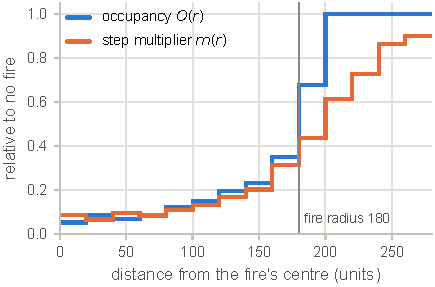
\includegraphics[width=0.52\linewidth]{figures/fire.pdf}
  \caption{Molotov profiles fitted on the training demos, relative to the same distances without a fire. The occupancy $O(r)$ weights the output belief; the step multiplier $m(r)$ reshapes the grid transitions. Both are 1 beyond 280~units.}
  \label{fig:fire}
\end{figure}

\subsection{Team coordination}
\label{sec:team}
The filters above track each enemy independently, so seeing three Terrorists on B says nothing about the other two. Real teams are strongly correlated. We correct each enemy's callout belief with recorded whole-team configurations. The \emph{team library} stores, every 2\,s of every training round, the callouts of each side's alive players together with the clock (round time before a plant, time since the plant after it), the bomb phase, the team's economy and the number alive: 133{,}726 snapshots.

At step $t$, let $k$ enemies be alive with callout beliefs $P_e$ (one-hot for an enemy on the radar). Candidate snapshots $q$ are those from the same side and bomb phase with at least $k$ players alive and a clock within 3\,s of the current one. Each gets a context weight
\begin{equation}
  \omega_q = \exp\!\Big(-\frac{(\kappa_q - \kappa_t)^2}{2 \cdot 2^2}\Big) \cdot 0.7^{|\mathrm{buy}_q - \mathrm{buy}|} \cdot 0.5^{\,n_q - k},
\end{equation}
where $\kappa$ is the clock and $n_q$ the snapshot's number of players. Let $\pi$ be the candidates' weighted callout occupancy. Each enemy's evidence enters as a likelihood ratio $r_e(k') \propto (P_e(k')/\pi(k'))^{\beta}$ with $\beta = 1$, normalized so that $\sum_{k'} \pi(k')\, r_e(k') = 1$. A snapshot's players are unlabelled, so we sum over every \emph{pairing} $s$, an injective map from our $k$ enemies to the $n_q$ recorded players (at most $5!/0! = 120$ pairings):
\begin{equation}
  W_{q,s} = \frac{\omega_q}{|\Sigma_{k,n_q}|} \prod_{e} r_e\big(c_{q,s(e)}\big), \qquad
  Q_e(k') = \frac{\sum_{q,s} W_{q,s}\, \1\big[c_{q,s(e)} = k'\big]}{\sum_{q,s} W_{q,s}},
  \label{eq:team}
\end{equation}
where $c_{q,j}$ is the callout of recorded player $j$ and $\Sigma_{k,n}$ is the set of pairings. $Q_e$ is enemy $e$'s callout distribution when the recorded teams are reweighted by how well they explain \emph{all} enemies' evidence at once. If recorded teammates were independent, the same computation would give $Q^{\mathrm{ind}}_e = \pi \cdot r_e \propto P_e$. We therefore apply only the ratio $R_e = \tilde Q_e / Q^{\mathrm{ind}}_e$, which is exactly 1 when recorded teams carry no information about correlations, and rescale each cell's belief by $R_e(c(i))$. To avoid over-reacting when few recorded teams match, $Q_e$ is shrunk towards the independent answer by credibility weighting \citep{buhlmann1967experience}: $\tilde Q_e = (n_{\mathrm{eff}} Q_e + \lambda Q^{\mathrm{ind}}_e)/(n_{\mathrm{eff}} + \lambda)$, where $n_{\mathrm{eff}} = (\sum_q W_q)^2 / \sum_q W_q^2$ is the effective number of recorded teams and $\lambda = 100$.

Summing over pairings marginalizes over the unknown correspondence between our enemies and the recorded players, much like joint probabilistic data association in multi-target tracking \citep{fortmann1983sonar}. The sum is a matrix permanent, which is hard to compute in general \citep{valiant1979complexity} but tiny here. The alternative of keeping only each snapshot's best pairing, which is what Hungarian matching would choose \citep{kuhn1955hungarian}, was clearly worse on validation. The correction is applied only once some enemy has been seen this round (\cref{sec:discussion} explains why).

\subsection{Calibration by time since last seen}
\label{sec:calibration}
Finally, the callout probabilities are passed through a monotone map fitted on the validation maps. For enemies last seen $\tau$ seconds ago, with $\tau$ in group $g$ (0--5\,s, 5--20\,s or 20\,s and longer),
\begin{equation}
  \tilde q(k) = \frac{\sigma\big(a_g \logit q(k) + b_g\big)}{\sum_{k'} \sigma\big(a_g \logit q(k') + b_g\big)},
  \label{eq:calib}
\end{equation}
where $\sigma$ is the logistic function. This is Platt scaling \citep{platt2000probabilities} applied to every callout and renormalized. It is increasing in $q$, so it never changes which callout ranks first, only how confident the model is. For small $q$, $\sigma(a \logit q + b) \approx e^{b} q^{a}$, so $a_g$ acts as an inverse temperature: $a > 1$ sharpens the distribution and $a < 1$ softens it. Each cell keeps its share of its callout, $b(i) \leftarrow b(i)\, \tilde q(c(i))/q(c(i))$. Enemies not yet seen this round are left unchanged. The map family and the grouping were chosen by 4-fold cross-validation over whole validation rounds (\cref{sec:res-calibration}). The fitted parameters are $(a_g, b_g) = (1.58, 1.61)$ for 0--5\,s, $(1.03, 0.46)$ for 5--20\,s and $(0.80, -0.04)$ beyond 20\,s: the raw filter is too unsure right after a sighting and too sure long after it.

\begin{algorithm}[t]
\caption{One step of the ensemble filter for a hidden enemy $e$. Lines 12--14 reshape only the reported belief.}
\label{alg:step}
\begin{algorithmic}[1]
\Require particles $\{(\ell_m, w_m)\}_{m=1}^{512}$, grid beliefs $h_{t-1}$ (\model{HMM}) and $p_{t-1}$ (\model{Prior+Neg}), information $\mathcal{I}_t$
\State $\ell_m \gets \mathrm{next}(\ell_m)$ for all $m$; re-match particles whose recording ended \Comment{predict}
\State $\bar h_t \gets h_{t-1}\, T^{(\varsigma,\phi_t,\tau_t)}$, with fire-blocked moves redirected; $\;\bar p_t \gets$ occupancy prior at round time $t$
\State $w_m \gets w_m\, L_t(\mathrm{cell}(\ell_m))\, K_t(\mathrm{cell}(\ell_m))$; $\;h_t \propto \bar h_t \odot L_t \odot K_t$; $\;p_t \propto \bar p_t \odot L_t \odot K_t$ \Comment{update}
\If{$e$ is on the radar in cell $j$}
  \State redraw every $\ell_m$ from library states near $j$ with probability $\propto \kappa(\ell)$ (\cref{eq:kernel})
  \State $w_m \gets 1/512$ for all $m$; $\;h_t \gets \delta_j$
\ElsIf{$1/\sum_m w_m^2 < 512/3$}
  \State systematic resampling; duplicates re-matched to fresh recordings
\EndIf
\State $h_t \gets (1 - 10^{-6})\, h_t + 10^{-6}/N$
\State $b_t \gets 0.75\, \mathrm{smooth}\big(\mathrm{hist}(\ell, w)\big) + 0.15\, h_t + 0.10\, p_t$
\State $b_t \gets$ team correction with $R_e$ (\cref{eq:team}), once any enemy has been seen \Comment{output only}
\State $b_t \gets \norm(b_t \odot O_t)$ while molotovs burn
\State $b_t \gets$ calibration of callout shares (\cref{eq:calib}) by the group of $\tau^e_t$
\State \Return $b_t$
\end{algorithmic}
\end{algorithm}

% ================================================================
\section{Experimental Setup}
\label{sec:setup}

\paragraph{Models.} We compare the full model (\model{Ens}) with the baselines of \cref{sec:motion}, with each motion model alone (\model{PF}, \model{HMM}), and with named ablations: \model{Ens$_0$}, the ensemble before the four late enhancements (molotovs, team coordination, calibration, and the tested but disabled weapon matching); versions without negative information (\model{PF}$-$neg, \model{HMM}$-$neg) or without the kill feed; and a copy of \model{Ens$_0$} with a different random seed, which measures Monte Carlo noise.

\paragraph{Evaluation moments.} A \emph{sample} is a (step, enemy) pair where the enemy is alive, off the radar, and was seen earlier in the round. Every round is scored from both teams' points of view, since each side is ``friendly'' once. The 16 HLTV test maps yield 102{,}486 samples in 315 rounds with at least one sample.

\paragraph{Metrics.} Let $k^\star$ be the callout and $i^\star$ the cell where the enemy really is.
\begin{itemize}
  \item \textbf{Callout top-1 / top-3:} whether $k^\star$ is the most likely callout, or among the three most likely; ties count against the model. Random guessing gets 4.3\% top-1.
  \item \textbf{Callout log-loss:} $-\ln q(k^\star)$, the average surprise at the truth in nats. It is minimized in expectation only by honest probabilities. A uniform guess over callouts scores $\ln 23 = 3.14$. The \emph{cell log-loss} $-\ln b(i^\star)$ is the same over cells (uniform: $\ln 1{,}999 = 7.60$).
  \item \textbf{Expected calibration error (ECE):} every callout probability of every sample is binned (edges 0, 0.05, 0.1, 0.2, \dots, 0.9, 1), and ECE is the bin-size-weighted mean of $|\text{mean stated probability} - \text{observed frequency}|$.
  \item \textbf{Team-level count error:} at each moment, the expected number of hidden enemies in each callout (the sum of their callout probabilities) is compared with the actual count, $\sum_k (\sum_e q^e(k) - n_k)^2$. This is a proper score for the expected counts.
\end{itemize}
Two readings of log-loss help build intuition. First, $e^{\LL}$ is the number of equally likely callouts the forecaster is effectively undecided between (its \emph{perplexity}). Second, log-loss has a betting interpretation. Suppose a bookmaker offers fair odds $1/q_B(k)$ on each callout according to model $B$, and a bettor using model $A$ spreads their bankroll over the callouts in proportion to $q_A$, the Kelly strategy for mutually exclusive outcomes. Their bankroll is multiplied by $q_A(k^\star)/q_B(k^\star)$ on each bet, so its expected logarithmic growth rate is exactly $\LL_B - \LL_A$ nats per bet \citep{kelly1956new,cover2006elements}.

\paragraph{Uncertainty.} Consecutive moments of a round are nearly the same situation, so the 102{,}486 samples are far from independent. All 95\% intervals come from a cluster bootstrap that resamples whole rounds, with 2{,}000 replicates \citep{field2007bootstrapping}. Both viewpoints of a round share a cluster. Model differences are \emph{paired}: in every replicate both models are scored on the same resampled rounds, so difficulty they share cancels, and a difference can be clearly nonzero even when the two models' separate intervals overlap. Particle filters are random, so we also compare two runs that differ only in their random seed; a claimed gain smaller than that difference is not a gain.

\paragraph{Protocol.} All settings (kernel widths, mixture weights, shrinkage strengths, calibration family) were chosen on validation data: the 8 HLTV validation maps, or the FACEIT validation matches during early development. The test maps were scored during development to track progress, but never used to choose a setting. All test results in \cref{sec:results} come from single evaluation runs of the final code and data.

% ================================================================
\section{Results}
\label{sec:results}

\subsection{Main results}
\label{sec:main}

\begin{table}[t]
\centering
\caption{Held-out professional test set: 16 HLTV maps, 102{,}486 samples of enemies seen earlier in the round and now off the radar. Round-bootstrap 95\% intervals in parentheses. Higher is better for accuracy, lower for log-loss.}
\label{tab:main}
\small
\setlength{\tabcolsep}{5pt}
\begin{tabular}{@{}lllll@{}}
\toprule
Model & Callout top-1 & Callout top-3 & Callout log-loss & Cell log-loss \\
\midrule
\model{Ens} (full model) & \textbf{0.482} \ci{0.457}{0.508} & 0.729 \ci{0.704}{0.754} & \textbf{1.663} \ci{1.580}{1.745} & \textbf{5.827} \ci{5.692}{5.952} \\
\model{Ens$_0$} (before enhancements) & 0.480 \ci{0.455}{0.506} & \textbf{0.730} \ci{0.705}{0.754} & 1.687 \ci{1.599}{1.774} & 5.854 \ci{5.711}{5.984} \\
\model{PF} (trajectory particles) & 0.475 \ci{0.451}{0.500} & 0.724 \ci{0.699}{0.748} & 1.867 \ci{1.741}{2.001} & 6.928 \ci{6.656}{7.203} \\
\model{HMM} (grid Markov chain) & 0.466 \ci{0.438}{0.495} & 0.704 \ci{0.674}{0.736} & 2.591 \ci{2.347}{2.838} & 7.060 \ci{6.753}{7.370} \\
\model{Diffuse} (random walk) & 0.444 \ci{0.417}{0.471} & 0.689 \ci{0.660}{0.720} & 3.023 \ci{2.743}{3.312} & 7.850 \ci{7.513}{8.191} \\
\model{LastSeen} & 0.422 \ci{0.394}{0.452} & 0.584 \ci{0.555}{0.613} & 7.196 \ci{6.834}{7.529} & 16.671 \ci{16.599}{16.738} \\
\model{Prior+Neg} & 0.215 \ci{0.193}{0.236} & 0.447 \ci{0.423}{0.470} & 2.609 \ci{2.552}{2.672} & 7.259 \ci{7.160}{7.363} \\
\model{Prior} & 0.213 \ci{0.192}{0.235} & 0.451 \ci{0.427}{0.475} & 2.607 \ci{2.550}{2.670} & 7.257 \ci{7.157}{7.361} \\
Uniform & -- & -- & 3.135 & 7.600 \\
\bottomrule
\end{tabular}
\end{table}

\Cref{tab:main} gives the headline comparison. The full model is the best in every metric except top-3, where \model{Ens$_0$} is 0.1 points ahead, well within noise. Against the last-seen heuristic, it names the right callout 6.1 points more often (paired 95\% interval 4.1 to 8.0) and has the right callout in its top three 14.5 points more often (12.3 to 16.7). Against the population prior the gains are 26.9 and 27.8 points. Its callout log-loss of 1.663 corresponds to a perplexity of $e^{1.663} \approx 5.3$ callouts, against 13.6 for the prior and 23 for a uniform guess. In the betting reading, a bankroll wagered according to \model{Ens} against a bookmaker pricing with \model{Prior} grows by a factor of $e^{0.94} \approx 2.6$ per bet on average (in the geometric sense). \model{LastSeen} has respectable accuracy but a catastrophic log-loss: it puts all its probability on one callout and is wrong 58\% of the time, so a Kelly bettor using it goes broke. Adding negative information and the kill feed to the prior changes almost nothing (\model{Prior+Neg} vs.\ \model{Prior}), because the prior does not know where the enemy was last seen.

\begin{table}[t]
\centering
\caption{What matters: paired differences on the test set (first model minus second), with round-bootstrap 95\% intervals. Positive $\Delta$top-1 and negative $\Delta$log-loss favour the first model. \model{HMM} is the learned grid chain, \model{PF} the replayed trajectories and \model{Diffuse} the untrained random walk; ``$-$neg'' removes negative information.}
\label{tab:ablation}
\small
\begin{tabular}{@{}llll@{}}
\toprule
Comparison & $\Delta$ callout top-1 & $\Delta$ callout log-loss & $\Delta$ cell log-loss \\
\midrule
\multicolumn{4}{@{}l}{\emph{Learned motion}} \\
\quad \model{HMM} vs.\ \model{Diffuse} & $+0.022$ \pd{+0.005}{+0.040} & $-0.432$ \pd{-0.558}{-0.308} & $-0.791$ \pd{-0.958}{-0.630} \\
\quad \model{PF} vs.\ \model{Diffuse} & $+0.031$ \pd{+0.012}{+0.048} & $-1.156$ \pd{-1.375}{-0.943} & $-0.923$ \pd{-1.161}{-0.678} \\
\quad \model{PF} vs.\ \model{HMM} & $+0.008$ \pd{-0.009}{+0.025} & $-0.724$ \pd{-0.901}{-0.559} & $-0.132$ \pd{-0.339}{+0.074} \\
\multicolumn{4}{@{}l}{\emph{Negative information}} \\
\quad \model{PF} vs.\ \model{PF}$-$neg & $+0.025$ \pd{+0.010}{+0.040} & $-0.042$ \pd{-0.080}{-0.005} & $-0.103$ \pd{-0.194}{-0.017} \\
\quad \model{HMM} vs.\ \model{HMM}$-$neg & $+0.015$ \pd{+0.006}{+0.024} & $-0.191$ \pd{-0.261}{-0.129} & $-0.245$ \pd{-0.317}{-0.179} \\
\multicolumn{4}{@{}l}{\emph{Ensemble and evidence}} \\
\quad \model{Ens$_0$} vs.\ \model{PF} (the mixture) & $+0.005$ \pd{-0.001}{+0.010} & $-0.180$ \pd{-0.251}{-0.124} & $-1.074$ \pd{-1.242}{-0.917} \\
\quad \model{Ens} vs.\ no kill feed & $+0.003$ \pd{-0.000}{+0.006} & $-0.010$ \pd{-0.015}{-0.004} & $-0.007$ \pd{-0.020}{+0.004} \\
\multicolumn{4}{@{}l}{\emph{Monte Carlo noise}} \\
\quad \model{Ens$_0$} vs.\ another seed & $+0.000$ \pd{-0.004}{+0.004} & $+0.004$ \pd{-0.003}{+0.012} & $+0.009$ \pd{-0.008}{+0.027} \\
\bottomrule
\end{tabular}
\end{table}

\subsection{What matters}
\label{sec:ablation}
\Cref{tab:ablation} isolates the components. \emph{Learned motion} is the largest single ingredient. Replaying recorded trajectories instead of a random walk cuts the callout log-loss by 1.16 nats, and it beats the learned grid chain by 0.72 nats while matching its accuracy. The chain's probabilities are badly spread: it often ranks the right callout first, but it assigns too little probability to where fast-moving players actually go. \emph{Negative information} improves every motion model, adding 2.5 points of accuracy to the particles and 1.5 to the grid chain. The \emph{mixture} of particles with the grid chain and the prior removes 0.18 nats of log-loss, and more than a nat of cell log-loss, by insuring against routes no particle took; its accuracy gain of 0.5 points is within noise. The kill feed gives a small but reliable log-loss gain; it matters because 48\% of killers are not on the radar at the moment of the kill. The seed comparison bounds Monte Carlo noise at about $\pm 0.004$ in accuracy and $\pm 0.01$ in callout log-loss on this test set. Validation ablations, not repeated on test, showed that conditioning the motion on the time since the last sighting was the largest single fix, roughly halving the cases where the true position received almost no probability, and that knowing the correct bombsite after the plant also helps.

\subsection{Accuracy as the trail goes cold}
\label{sec:horizon}

\begin{figure}[t]
  \centering
  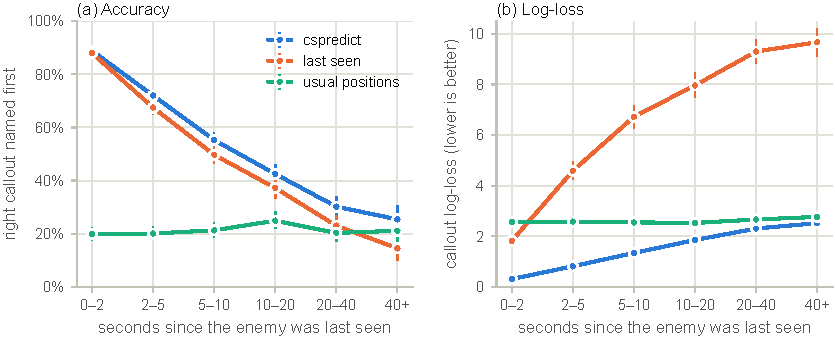
\includegraphics[width=\linewidth]{figures/horizon.pdf}
  \caption{Test-set accuracy and log-loss by time since the enemy was last seen, with round-bootstrap 95\% intervals. ``Usual positions'' is \model{Prior+Neg}. Each bin holds 11{,}256 to 23{,}229 samples.}
  \label{fig:horizon}
\end{figure}

\Cref{fig:horizon} breaks the results down by the time since the last sighting (full table in \cref{app:tables}). In the first two seconds most enemies have not left their callout, so \model{Ens} and \model{LastSeen} are nearly tied in accuracy (88.8\% vs.\ 88.0\%), but the model's log-loss is six times lower (0.31 vs.\ 1.82) because it hedges the remaining cases. The gap then widens: 42.5\% against 37.2\% at 10--20\,s, and 25.4\% against 14.5\% after 40\,s. By 20--40\,s, \model{LastSeen} is barely better than the population prior (23.0\% vs.\ 20.3\%), and after 40\,s it is worse (14.5\% vs.\ 21.1\%), while the model stays above both. Its log-loss rises smoothly towards the prior's as the information ages, never exceeding it. This is the behaviour one wants from a forecaster that knows what it does not know.

\subsection{Clutch situations}
\label{sec:clutch}
Rounds often end with one player left against several (a ``clutch''), and these are the moments where a coach most wants to know what the lone player could have inferred. \Cref{tab:clutch} shows callout accuracy from the lone player's side. The model's lead over \model{LastSeen} is largest in the 1-versus-1 (59.9\% vs.\ 42.5\%), where a single opponent's movement dominates. Each slice contains only 40 to 98 rounds, so differences of a point or two between \model{Ens} and \model{Ens$_0$} are within noise. Against four or five opponents, the full model's log-loss is clearly better than \model{Ens$_0$}'s ($-0.040$ and $-0.036$ nats).

\begin{table}[t]
\centering
\caption{Callout top-1 accuracy when one friendly player is left (test set), by the number of enemies alive. Callout log-loss of \model{Ens} in the last row.}
\label{tab:clutch}
\small
\begin{tabular}{@{}lccccc@{}}
\toprule
 & 1v1 & 1v2 & 1v3 & 1v4 & 1v5 \\
\midrule
Samples & 2{,}001 & 4{,}292 & 5{,}963 & 8{,}701 & 3{,}179 \\
\model{Ens} & \textbf{0.599} & 0.514 & 0.483 & \textbf{0.390} & \textbf{0.412} \\
\model{Ens$_0$} & 0.596 & \textbf{0.521} & \textbf{0.493} & 0.378 & 0.407 \\
\model{LastSeen} & 0.425 & 0.421 & 0.376 & 0.343 & 0.394 \\
\model{Prior+Neg} & 0.361 & 0.349 & 0.304 & 0.157 & 0.131 \\
\midrule
\model{Ens} callout log-loss & 1.326 & 1.634 & 1.599 & 2.025 & 1.835 \\
\bottomrule
\end{tabular}
\end{table}

\subsection{Calibration}
\label{sec:res-calibration}

\begin{table}[t]
\centering
\caption{Choosing the calibration map: 4-fold cross-validated callout log-loss of \model{Ens} before calibration, on the 8 validation maps (63{,}906 samples, 166 rounds; folds are whole rounds). ``By horizon'' fits separate parameters for 0--5\,s, 5--20\,s and 20\,s and longer since the last sighting.}
\label{tab:calib-cv}
\small
\begin{tabular}{@{}lcc@{}}
\toprule
Map family & One map for all moments & By horizon \\
\midrule
None & 1.6890 & -- \\
Power (temperature scaling), 1 parameter & 1.6871 & 1.6680 \\
Platt (logit-affine), 2 parameters & 1.6859 & \textbf{1.6660} \\
Piecewise linear in $\log q$, 4 parameters & 1.6824 & 1.6681 \\
\bottomrule
\end{tabular}
\end{table}

\Cref{tab:calib-cv} shows how the calibration map was chosen. A single map for all moments barely helps (at best $-0.007$ nats), because the raw model errs in opposite directions at different horizons. Fitting separate maps by the time since the last sighting gains about three times as much ($-0.021$ to $-0.023$, depending on the family). \Cref{fig:calibration} shows why on the test set. Within 5\,s of a sighting the raw ensemble is \emph{under}-confident (above the diagonal), because its 10\% population-prior component caps how sure it can be. Across all horizons, its most confident bin claimed 92\% on average and was right 98.5\% of the time. After 20\,s it is \emph{over}-confident: stated probabilities averaging 44\% and 54\% came true only 37\% and 47\% of the time. On the test set the calibrated model's calibration error falls from 0.0040 to 0.0010 overall, and in every horizon group (\cref{fig:calibration}). \Cref{tab:reliability} lists the overall reliability. Calibration left top-1 accuracy unchanged by construction and improved the callout log-loss by 0.020 nats (paired interval 0.010 to 0.031).

\begin{figure}[t]
  \centering
  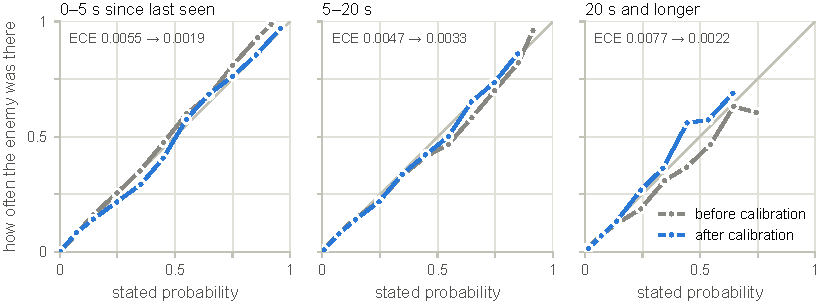
\includegraphics[width=\linewidth]{figures/calibration.pdf}
  \caption{Reliability of the callout probabilities on the test set, by time since the enemy was last seen, before and after calibration. A perfectly calibrated forecaster lies on the diagonal. Every callout probability of every sample is binned; bins with fewer than 200 probabilities are omitted. ECE: expected calibration error.}
  \label{fig:calibration}
\end{figure}

\begin{table}[t]
\centering
\caption{When the model states a callout probability in a given range, how often the enemy was really there (test set, all horizons).}
\label{tab:reliability}
\small
\setlength{\tabcolsep}{4.5pt}
\begin{tabular}{@{}lcccccccc@{}}
\toprule
Stated & 20--30\% & 30--40\% & 40--50\% & 50--60\% & 60--70\% & 70--80\% & 80--90\% & 90\%+ \\
\midrule
Before calibration & 20.7\% & 32.4\% & 40.8\% & 50.2\% & 62.3\% & 74.5\% & 89.0\% & 98.5\% \\
After calibration & 24.0\% & 33.7\% & 43.8\% & 53.3\% & 66.4\% & 74.8\% & 85.7\% & 97.0\% \\
\bottomrule
\end{tabular}
\end{table}

\subsection{The four enhancements}
\label{sec:enhancements}
The ensemble \model{Ens$_0$} was extended in four steps, each tested on validation first. \Cref{tab:enhance} reports each step's paired effect on test relative to the step before, together with the subset of moments where the step is designed to act. Overall, \model{Ens} improves on \model{Ens$_0$} by 0.024 nats of callout log-loss (0.012 to 0.036) and 0.027 of cell log-loss (0.015 to 0.040); its top-1 gain of $+0.002$ ($-0.001$ to $+0.006$) is within noise. Most of the gain is concentrated where each step should act: molotovs help while a fire burns (19\% of samples), and the team correction helps enemies nobody has seen yet once one of their teammates has been. In the betting reading, 0.024 nats is a bankroll growing by about 2.4\% per bet against the earlier model.

\begin{table}[t]
\centering
\caption{Paired effect of each enhancement on the test set, relative to the step before (95\% round-bootstrap intervals), and where it shows.}
\label{tab:enhance}
\small
\setlength{\tabcolsep}{4pt}
\begin{tabular}{@{}>{\raggedright\arraybackslash}p{2.55cm}lll>{\raggedright\arraybackslash}p{4.0cm}@{}}
\toprule
Step & $\Delta$ top-1 & $\Delta$ callout LL & $\Delta$ cell LL & Where it shows \\
\midrule
Weapon at last sighting (tested, left off) & $-0.002$ \pd{-0.006}{+0.000} & $-0.002$ \pd{-0.010}{+0.005} & $-0.014$ \pd{-0.032}{+0.003} & Nowhere beyond Monte Carlo noise \\[2pt]
Molotovs & $+0.001$ \pd{-0.000}{+0.002} & $-0.001$ \pd{-0.002}{+0.000} & $-0.004$ \pd{-0.007}{-0.002} & While a fire burns: top-1 $+0.005$ \pd{+0.001}{+0.010}, cell LL $-0.017$ \pd{-0.026}{-0.006} \\[2pt]
Team coordination & $+0.002$ \pd{-0.001}{+0.005} & $-0.003$ \pd{-0.008}{+0.003} & $-0.003$ \pd{-0.008}{+0.003} & Never-seen enemies after first contact: top-1 $+0.017$ \pd{+0.011}{+0.022}, LL $-0.031$ \pd{-0.040}{-0.022}; count error $-0.020$ \pd{-0.033}{-0.007} \\[2pt]
Calibration & 0 (by design) & $-0.020$ \pd{-0.031}{-0.010} & $-0.020$ \pd{-0.031}{-0.010} & Reliability (\cref{fig:calibration}) \\
\bottomrule
\end{tabular}
\end{table}

\subsection{Coordination and the team as a whole}
\label{sec:res-team}
The test set contains 246{,}193 samples of enemies who have not been seen yet in the round while at least one of their teammates has. For these, the team correction raises top-1 accuracy from 0.176 to 0.193 and lowers callout log-loss from 2.609 to 2.578. That brings the model level with \model{Prior+Neg} (0.191, 2.600) on enemies it has no direct evidence about, which the independent filters could not reach. At the team level, the expected number of hidden enemies per callout misses the actual count by a squared error of 2.908 per moment after first contact (2.787 to 3.035), against 2.931 for the independent filters and 3.264 for the prior. The model still underestimates stacks: where it expects 1.5--2 enemies in one callout there are 1.96 on average, and where it expects 2--3 (mean 2.26) there are 2.49.

Two design details mattered on validation. Summing over all pairings (\cref{eq:team}) beat keeping each snapshot's single best pairing by a wide margin. And applying the correction before first contact \emph{hurt}. With no sightings, every enemy's belief is the same, so the product in \cref{eq:team} multiplies five copies of one likelihood ratio and counts the shared negative evidence five times.

\subsection{Training data: more versus purer}
\label{sec:res-data}
\Cref{tab:sources} compares models trained on the FACEIT matches, the professional matches, or both, all scored on the professional test set before calibration so that they are compared alike. Pooling the 35 FACEIT matches with the 47 professional ones beats the professional matches alone by 1.2 points of accuracy (0.2 to 2.1) and 0.043 nats of log-loss (0.023 to 0.063). For this model, more data beats purer data.

\begin{table}[t]
\centering
\caption{Effect of the training data on the professional test set (\model{Ens} before calibration).}
\label{tab:sources}
\small
\begin{tabular}{@{}lccc@{}}
\toprule
Trained on & Callout top-1 & Callout log-loss & Cell log-loss \\
\midrule
FACEIT only (35 maps) & 0.463 & 1.761 & 6.162 \\
HLTV only (47 maps) & 0.470 & 1.726 & 5.944 \\
Both (82 maps) & \textbf{0.482} & \textbf{1.684} & \textbf{5.847} \\
\bottomrule
\end{tabular}
\end{table}

\subsection{The FACEIT development set}
\label{sec:res-faceit}
On the 6 FACEIT test matches (48{,}876 samples), with models trained and calibrated on FACEIT data only, \model{Ens} reaches 0.463 top-1 \ci{0.430}{0.499} and 1.731 callout log-loss \ci{1.611}{1.849}, against 0.378 and 7.834 for \model{LastSeen} and 0.219 and 2.603 for \model{Prior}. The four enhancements improve log-loss by 0.063 nats (0.043 to 0.082), more than on professional matches. Professional play is more predictable. \model{LastSeen} alone is right 42\% of the time on professional matches but only 38\% on FACEIT, because professionals hold positions more, and in 1-versus-1 clutches \model{Ens} names the right callout 60\% of the time on professional matches but only 24\% on FACEIT.

\subsection{Features that did not help}
\label{sec:negative}
We report these because each was a plausible hypothesis, and several are features a knowledgeable player would suggest first.
\begin{itemize}
  \item \textbf{The weapon in hand at the last sighting.} The signal is real: AWP snipers move less in the 5\,s after being seen (median 190 vs.\ 300 units for riflers), and players seen holding a knife or grenade move more. Yet matching on the weapon, whether on every weapon class, on guns only, or on AWP versus the rest, never beat Monte Carlo noise on validation or on test (\cref{tab:enhance}). Over 80\% of sightings are rifles or pistols, where the weapon mostly repeats what position and economy already say.
  \item \textbf{Man advantage and player identity.} Matching trajectories on the numbers alive on each side (1v3 plays differently from 5v5), or preferring the same player's own recordings, did not help on the FACEIT validation data. Even soft versions left too few matching trajectories. Both are implemented but disabled, and they have not been re-tested on professional data.
  \item \textbf{Molotovs inside the particle filter.} Making particles wait at a fire's edge failed, because real players often re-route, so waiting particles fell out of step with their recordings. Re-weighting particles by the occupancy profile at every step counted one standing fact as a new observation at every step. Both were slightly worse, within noise. Only the grid-level and output-level versions are used.
  \item \textbf{Flashed teammates.} A flashed player really does stop spotting, from about a quarter of the flash duration until 1.25 times it. However, only one mid- or late-round moment in eight has a teammate flashed now or in the previous 5\,s, and rebuilding the flashes missing from 55 HLTV demos moved validation log-loss by only $-0.001$ ($-0.006$ to $+0.005$). The gain is confined to the 5\,s after a flash, where cell log-loss improves by 0.029 (0.003 to 0.062).
  \item \textbf{Smoke timing.} Fixing the parsing bug that cut 15\% of smokes 4\,s short initially made results slightly worse. It helped only once smokes were also treated as see-through for their last 1.5\,s, which matches when spotting through them resumes in the data.
\end{itemize}

\subsection{Comparison with a general-purpose model}
\label{sec:jev}
Can a general-purpose model do the same job given the same information? We queried TypeSafe's Jev (\texttt{jev-1.13.0}; \citealp{typesafe2026}), a hosted model that answers multiple-choice questions posed as text with a probability for every option. For each hidden enemy it was asked which of the 23 callouts the enemy is in. It received a structured description of only what the team knew, and it never saw later events, true positions or our model's beliefs. Facts computed in code were labelled as such: travel times from the last sighting, spotting coverage per callout, and base rates from the \emph{training} rounds. Every variant was developed on 2{,}000 validation moments; then all variants were run once on 3{,}000 test moments. Calibration, blend weights and a simple baseline formula were fitted on validation.

\begin{table}[t]
\centering
\caption{A general-purpose model on 3{,}000 held-out professional moments (a random subset of the test samples). The last column is how often the top pick is the callout where the enemy was last seen; the enemy really was still there in 42\% of these moments.}
\label{tab:jev}
\small
\begin{tabular}{@{}lcccc@{}}
\toprule
Model & Callout top-1 & Top-3 & Log-loss & Picks last-seen callout \\
\midrule
\cs{} (\model{Ens}) & \textbf{0.489} \ci{0.459}{0.522} & \textbf{0.739} & \textbf{1.648} & 59\% \\
Formula: 9 weights on the same facts, no Jev & 0.457 \ci{0.425}{0.490} & 0.710 & 1.819 & 75\% \\
Jev, split questions + movement rates, calibrated & 0.416 \ci{0.387}{0.449} & 0.703 & 1.944 & 40\% \\
Jev, split questions, calibrated & 0.416 & 0.683 & 2.023 & 75\% \\
Jev, focused per-enemy questions, calibrated & 0.419 & 0.642 & 2.038 & 86\% \\
Jev, plain description + travel times, calibrated & 0.404 & 0.629 & 2.182 & 76\% \\
Jev, plain description, calibrated & 0.406 \ci{0.375}{0.443} & 0.605 & 2.180 & 84\% \\
Jev, plain description, raw & 0.406 & 0.605 & 4.066 & 84\% \\
\model{LastSeen} & 0.420 \ci{0.388}{0.455} & 0.584 & 7.150 & 100\% \\
\model{Prior} & 0.233 & 0.466 & 2.589 & 19\% \\
\bottomrule
\end{tabular}
\end{table}

\Cref{tab:jev} shows the results. Given a plain description, the model mostly repeats the last sighting (84\% of its top picks), its accuracy is no better than \model{LastSeen}, and its raw probabilities are over-confident (log-loss 4.07). A two-parameter calibration per horizon group halves that log-loss. Following the vendor's own advice (focused per-enemy questions, facts computed in code, and splitting ``which callout?'' into ``still there?'' and ``if not, where?'') improved its probabilities step by step. Supplying movement rates from the training rounds (of the players last seen in that callout that long ago, the share still there and where the others went) finally broke the anchoring: its last-seen rate fell to 40\%, close to the true 42\%, and its top-3 accuracy rose by 9.8 points (7.8 to 11.6) over the plain variant. Its top-1 accuracy still only ties \model{LastSeen} ($-0.003$; $-0.035$ to $+0.030$), and a 9-parameter formula on the same facts beats it by 4.1 points (1.1 to 6.9). Blending 20\% of Jev into that formula improves log-loss by 0.034 (0.020 to 0.049), so the model extracts something the formula misses, but not much. All experiments together cost about US\$2.60 in API calls.

% ================================================================
\section{Discussion}
\label{sec:discussion}

\paragraph{Why replayed trajectories beat a Markov chain.} A first-order chain's next position depends only on its current cell, so it cannot represent momentum: a player sprinting down a corridor is modelled as equally likely to turn back at every step. The belief therefore spreads like a diffusing cloud, growing roughly as the square root of time, while real players move \emph{ballistically} along routes until they stop, covering distance in proportion to time. Replaying recorded trajectories preserves momentum, route choice and typical stopping points, and it represents the branching into distinct routes directly. The price is sampling noise and the risk that no particle took the route the enemy chose, which the defensive mixture with the grid chain and the prior covers (\cref{tab:ablation}). This mirrors the classical trade-off between analog and model-based forecasting \citep{lorenz1969atmospheric}.

\paragraph{The power and the danger of negative information.} Absence of evidence is the most abundant evidence in this problem, and treating it properly improves every model. But \cref{eq:neg} is applied every 0.25\,s under an independence assumption. If the spotting model wrongly believes a cell is visible, the error compounds across steps, and the filter can become confident that the enemy is not somewhere it is. The 0.9 cap on $\pi_o$, the uniform floor and the mixture components all limit this. One plausible contributor to the late-horizon over-confidence of \cref{fig:calibration} is exactly this accumulation of correlated negative evidence; the calibration corrects the symptom, not the cause.

\paragraph{Counting evidence once.} Two of our design lessons are instances of one principle. Bayes' rule assumes that each observation is new. Re-weighting particles by a burning fire at every step treats one standing fact as dozens of independent observations. Applying the team correction before first contact multiplies five identical copies of the same evidence. In both cases the fix was to apply the information exactly once: fire occupancy only on the output, and the team correction only after sightings make the enemies' beliefs distinct.

\paragraph{Why calibration must depend on the horizon.} The raw ensemble's miscalibration has two sources that dominate at opposite ends. Just after a sighting, the probability held by the blunt mixture components, above all the 10\% population prior, makes the model under-confident. Long after it, compounded negative evidence and particle degeneracy make it over-confident. A single global map must compromise between the two, which is why it helped so little (\cref{tab:calib-cv}), while horizon-specific maps fixed both.

\paragraph{When a real signal adds nothing.} The weapon result is a reminder that a variable can be correlated with the outcome and still add no information beyond what the model already conditions on. Here, position and economy largely determine which weapon a player carries and how they play. Man-advantage matching failed for a different reason: every extra matching variable divides the pool of similar recorded trajectories, and with a few dozen training maps (35 FACEIT maps when this was tested) the pool runs dry, the familiar curse of dimensionality \citep{bellman1961adaptive}.

\paragraph{Structure versus generality.} The general-purpose model anchored on the most salient cue, the last sighting, until it was handed movement statistics that the structured model learns directly. Even then, a nine-parameter formula on the same facts did better. With a few dozen matches of training data, building the structure of the problem into the model (motion, sight lines, Bayes' rule) is far more data-efficient than asking a general model to infer it.

% ================================================================
\section{Limitations and Ethical Considerations}
\label{sec:limitations}

\paragraph{Scope and data.} Everything is learned per map, and we have studied one map with 71 professional and 46 FACEIT matches. The 16 test maps give intervals of about $\pm 2.5$ points on top-1 accuracy. Teams recur across the train/test split, so the results measure generalization to new matches, not to unseen teams. Most professional teams in the data are tier two or three.

\paragraph{Information left out.} Sound (footsteps, gunshots, reloads) is not used, by choice. It is probably the largest source of information a real team has that the model ignores, and including it is the most promising extension. We also assume enemies are identifiable on the radar and that molotovs are common knowledge.

\paragraph{Modelling approximations.} Coordination enters as a correction on top of independent filters rather than as a joint model, and the model still underestimates how many enemies stack in one callout. The geometry is learned from where players stand, so windows and rarely walked spots are approximate; exact geometry would improve the spotting model. Blinding is modelled from 0 to 1 times the flash duration, whereas the data suggest a window from about 0.25 to 1.25 times; that refinement is untested.

\paragraph{Fair play.} A live overlay built on this model would show players information beyond what the game gives them. Competitive platforms prohibit third-party software that gives an unfair advantage \citep{faceit2026cheat}, and \citet{hladky2008evaluation} noted that such an overlay would be nearly undetectable, which makes the rule more important, not less. We built and evaluated \cs{} strictly for post-match review, coaching and analysis. Uses such as broadcast graphics, bot behaviour, or anti-cheat research, which could flag players who act on information they should not have, are compatible with that intent.

% ================================================================
\section{Conclusion}
\label{sec:conclusion}
We have shown that the reasoning players and coaches do about unseen opponents in Counter-Strike~2 can be made quantitative, calibrated and testable. A Bayes filter built entirely from recorded matches, with a learned map, a learned spotting model, and particles that replay recorded trajectories, names the right callout for a hidden opponent 48\% of the time, with probabilities that mean what they say. The gains come mostly from two ideas that are old in filtering but new to this setting: negative information and analog motion. Coordination between opponents and horizon-dependent calibration add smaller, targeted improvements, and several intuitive features add nothing. Natural next steps are sound, more maps and seasons, joint models of whole teams, and learned motion models such as those of \citet{durst2024learning} inside the same probabilistic framework.

\section*{Acknowledgments}
We thank the authors of the X-Ego-CS dataset for releasing their recordings under the MIT license, HLTV.org for hosting professional demos, and the maintainers of demoparser2 and awpy. The software and this manuscript were developed with the assistance of an AI coding assistant (Claude, Anthropic).

\bibliographystyle{plainnat}
\bibliography{references}

% ================================================================
\clearpage
\appendix

\section{Hyperparameters}
\label{app:hyper}

\begin{table}[H]
\centering
\caption{Constants of the final model. Unless noted, values were set once and checked on validation.}
\label{tab:hyper}
\small
\begin{tabularx}{\linewidth}{@{}lX@{}}
\toprule
Component & Setting \\
\midrule
Sampling & 64-tick demos stored at 8\,Hz; filter step 0.25\,s (16 ticks) \\
Grid & 64-unit columns; floors split at a 110-unit height gap; a floor needs 8 samples (1\,s); step edges up to 48 units; 16-unit raster for ray casting \\
Spotting model & 8 distance bins; 36 horizontal and 10 vertical 5$^\circ$ bins; 3 sight-line classes; $L_2$ penalty $0.005\|w\|^2$; rays sampled every 8 units up to 4{,}500; eye height 64, chest 48; smoke radius 130; pair correction with 3 pseudo-counts, clipped to $[0.02, 50]$; $\pi_o \le 0.9$ \\
Information state & smoke blocks from $+1.0$\,s after burst to $-1.5$\,s before expiry; molotov burns from $+0.5$\,s; blind if flash $> 0.3$\,s; economy edges 1{,}500 and 3{,}800 \\
Economy estimate & 11 situations with 3 pseudo-rounds at the overall frequencies; gun likelihoods with add-one smoothing, exponent 0.7 (fitted on training rounds) \\
Negative information & $\gamma = 1$ \\
Kill feed & $K = 0.05 + 0.95\,\tilde\pi/\max\tilde\pi$; wallbang or smoke: 1 within 2{,}000 units, else 0.05 \\
Grid chain & time-since-seen bins 0--2, 2--5, 5--10, 10--20, 20+\,s and never; smoothing 0.5; shrinkage 4 pseudo-counts \\
Particles & $M = 512$; $\ge 40$ candidates (widen up to 3 rings); round-time kernel $\sigma = 15$\,s; other bomb phase $\times 0.02$; time-since-seen kernel $\sigma = 0.5$ in $\ln(1 + \tau)$, seen/never mismatch $\times 0.05$; economy $\times 0.7$ per level; heading von Mises $\kappa = 3$ above 80 units/s; resample when ESS $< M/3$; smoothing weights 0.4 / 0.4 / 0.2 \\
Ensemble & 0.75 particles, 0.15 grid chain, 0.10 prior with negative information; uniform floor $10^{-6}$ \\
Prior & 5-s round-time bins by side and bomb phase; 0.01 pseudo-count per cell \\
Molotovs & 20-unit bins to 280; same floor within 100 units; control window from 1\,s after burnout; step profile bounded to $[0.01, 1]$ \\
Team correction & snapshots every 2\,s; clock $\sigma = 2$\,s, window $\pm 3$\,s; economy $\times 0.7$ per level; $\times 0.5$ per extra recorded player; $\beta = 1$; probability floor $10^{-3}$; shrinkage $\lambda = 100$; at most 5{,}000 candidates; only after first contact \\
Calibration & Platt map per horizon group (0--5, 5--20, 20+\,s): $(a, b) = (1.58, 1.61), (1.03, 0.46), (0.80, -0.04)$ \\
\bottomrule
\end{tabularx}
\end{table}

\section{Additional Results}
\label{app:tables}

\begin{table}[H]
\centering
\caption{Test-set callout top-1 and callout log-loss by time since the last sighting (the data of \cref{fig:horizon}).}
\label{tab:horizon}
\small
\begin{tabular}{@{}llcccccc@{}}
\toprule
 & & 0--2\,s & 2--5\,s & 5--10\,s & 10--20\,s & 20--40\,s & 40\,s+ \\
\midrule
 & Samples & 11{,}256 & 14{,}004 & 16{,}612 & 21{,}292 & 23{,}229 & 16{,}093 \\
\midrule
\multirow{4}{*}{Top-1} & \model{Ens} & 0.888 & \textbf{0.720} & \textbf{0.553} & 0.425 & \textbf{0.302} & \textbf{0.254} \\
 & \model{Ens$_0$} & \textbf{0.889} & 0.716 & 0.546 & \textbf{0.429} & 0.297 & 0.251 \\
 & \model{LastSeen} & 0.880 & 0.675 & 0.497 & 0.372 & 0.230 & 0.145 \\
 & \model{Prior+Neg} & 0.199 & 0.201 & 0.213 & 0.249 & 0.203 & 0.211 \\
\midrule
\multirow{4}{*}{Log-loss} & \model{Ens} & \textbf{0.308} & \textbf{0.812} & \textbf{1.340} & \textbf{1.849} & \textbf{2.305} & \textbf{2.515} \\
 & \model{Ens$_0$} & 0.365 & 0.830 & 1.355 & 1.857 & 2.345 & 2.526 \\
 & \model{LastSeen} & 1.815 & 4.587 & 6.723 & 7.962 & 9.300 & 9.669 \\
 & \model{Prior+Neg} & 2.565 & 2.576 & 2.548 & 2.525 & 2.661 & 2.765 \\
\bottomrule
\end{tabular}
\end{table}

\subsection{Improper scores favour over-confidence}
\label{app:improper}
\Cref{tab:improper} scores the same test samples with two intuitive but improper measures: the probability placed within 300 walking units of the true position, and the expected walking distance from the belief to the truth. By both, \model{LastSeen} looks better than the full model. Both measures reward concentrating probability on a single point, whether or not that concentration is justified. A forecaster optimizing them would report over-confident beliefs. This is why the paper's conclusions rest on log-loss and accuracy.

\begin{table}[H]
\centering
\caption{Improper scores on the test set (higher is better for mass within 300 units, lower for expected distance). They rank the models differently from the proper log-loss.}
\label{tab:improper}
\small
\begin{tabular}{@{}lccc@{}}
\toprule
Model & Mass within 300 units & Expected distance (units) & Callout log-loss (proper) \\
\midrule
\model{Ens} & 0.274 & 1{,}100 & \textbf{1.663} \\
\model{PF} & 0.287 & 1{,}022 & 1.867 \\
\model{HMM} & 0.319 & 916 & 2.591 \\
\model{Diffuse} & 0.300 & 902 & 3.023 \\
\model{LastSeen} & \textbf{0.339} & \textbf{855} & 7.196 \\
\model{Prior} & 0.045 & 1{,}923 & 2.607 \\
\bottomrule
\end{tabular}
\end{table}

\subsection{Team-level counts}
\begin{table}[H]
\centering
\caption{Expected against actual numbers of hidden enemies in a callout, after first contact (test set, \model{Ens}), binned by the expected number. The model is accurate for sparse callouts and underestimates stacks.}
\label{tab:counts}
\small
\begin{tabular}{@{}lccccccc@{}}
\toprule
Model expects & 0--0.1 & 0.1--0.25 & 0.25--0.5 & 0.5--0.75 & 0.75--1 & 1--1.5 & 1.5--2 \\
\midrule
Mean expected & 0.029 & 0.161 & 0.347 & 0.613 & 0.858 & 1.174 & 1.688 \\
Mean actual & 0.031 & 0.158 & 0.340 & 0.588 & 0.843 & 1.313 & 1.957 \\
\bottomrule
\end{tabular}
\end{table}

\section{Reproducibility}
\label{app:repro}
All results can be regenerated from the demo files with the project's command-line tools (Python~3.12):
{\footnotesize
\begin{verbatim}
python -m cspredict.parse                        # demos -> parquet tables
python -m cspredict.build --sources hltv xego    # grid, spotting, motion, fires, teams, economy
python -m cspredict.evaluate --train-sources hltv xego --sources hltv \
    --split val --models ens_uncal --out outputs/final/val_pooled_uncal
python -m cspredict.calibrate --train-sources hltv xego \
    --run outputs/final/val_pooled_uncal --model ens_uncal
python -m cspredict.evaluate --train-sources hltv xego --sources hltv --split test \
    --models last_seen prior prior_neg diffuse hmm_noneg hmm pf_noneg pf \
             ens ens_nokill ens_uncal ens_indep ens_nofire ens_w0.5 ens_seed1 \
    --ref ens_nofire --focus last_seen prior_neg ens_nofire ens --out outputs/final/test_pooled
python paper/make_figures.py                     # figures and the paired comparisons
\end{verbatim}
}
The training-data comparison (\cref{tab:sources}) and the FACEIT results repeat the build, calibrate and evaluate steps with \texttt{--sources hltv} or \texttt{--sources xego}; the Jev benchmark is \texttt{python -m cspredict.jev\_lab} (see \texttt{docs/jev.md}). Model names in the code map to the paper as follows: \texttt{ens} is \model{Ens}, \texttt{ens\_nofire} is \model{Ens$_0$}, \texttt{pf} and \texttt{hmm} are \model{PF} and \model{HMM}, \texttt{diffuse}, \texttt{last\_seen}, \texttt{prior} and \texttt{prior\_neg} are the baselines, and the suffix \texttt{\_noneg} removes negative information.

The comparison with the true economy class in \cref{sec:problem} uses \texttt{ens\_truebuy} and \texttt{ens\_truebuy\_seed1} on validation, which take the class from the recorded equipment values, and on test the calibrated model of earlier versions (git commit \texttt{66a5aeb}).

\end{document}
